\documentclass[10pt]{article}
\usepackage[utf8]{inputenc}
\usepackage[T1]{fontenc}
\usepackage{amsmath}
\usepackage{amsfonts}
\usepackage{amssymb}
\usepackage[version=4]{mhchem}
\usepackage{stmaryrd}
\usepackage{graphicx}
\graphicspath{ {./images/} }
\usepackage{tikz,lipsum,lmodern}
\usepackage[most]{tcolorbox}
\usepackage{multicol} 


\title{Homework 0 }

\author{Fardeen Azizi}


\begin{document}
\maketitle

\section*{1)}

Let $\mathrm{A}$ be the event I test positive, let $\mathrm{B}$ be the event I have the disease.

We are solving for the probability that I have the disease, given that I tested positive.

Using Bayes Theorem:

$$
P(B \mid A)=\frac{P(A \mid B) * P(B)}{P(A)}
$$

Applying the law of total probability to $\mathrm{P}(\mathrm{A})$ :

$$
P(B \mid A)=\frac{P(A \mid B) * P(B)}{P(A \mid B) P(B)+P\left(A \mid B^{c}\right) P\left(B^{c}\right)}
$$

Substituting in values we are given:

$$
P(B \mid A)=\frac{0.99 * 0.0001}{0.99 * 0.0001+P\left(A \mid B^{c}\right) * 0.9999}
$$

To solve for $P\left(A \mid B^{c}\right)$, we solve for it's completement which is $1-P\left(A^{c} \mid B^{c}\right)$ where $P\left(A^{c} \mid B^{c}\right)$ given in the problem as 0.99 . Inputting this in:

$$
\frac{0.99 * 0.0001}{0.99 * 0.0001+0.01 * 0.9999}
$$

\begin{tcolorbox}[colback=red!5!white,colframe=red!75!black]
  \centering Answer: $P(B \mid A)=0.0098$
\end{tcolorbox}
\newpage

\section*{2)}

A)

$$
\begin{gathered}
\operatorname{Cov}(X, Y)=E[(X-E[X])(Y-E[Y])] \\
=E[(X Y-X E[Y]-Y E[X]+E[X] E[Y])]
\end{gathered}
$$

Using linearity of expectation we get:

$$
\begin{gathered}
=E[X Y]-E[X] E[Y]-E[Y] E[X]+E[X] E[Y] \\
=E[X Y]-E[Y] E[X]
\end{gathered}
$$

Using the law of total expectation:

Expanding this:

$$
=E[E[X Y \mid X]]-E[E[Y \mid X]] E[X]
$$

$$
=\sum_{x_{i} \in \Omega_{X}} E\left[X Y \mid X=x_{i}\right] P\left(X=x_{i}\right)-E[X] \sum_{x_{i} \in \Omega_{X}} E\left[Y \mid X=x_{i}\right] P\left(X=x_{i}\right)
$$

Using the definition given in the problem and how $X=x_{i}$, we get:

Therefore:

$$
\begin{gathered}
=\sum_{x_{i} \in \Omega_{X}} E\left[x_{i} Y \mid X=x_{i}\right] P\left(X=x_{i}\right)-E[X] \sum_{x_{i} \in \Omega_{X}} x_{i} * P\left(X=x_{i}\right) \\
=\sum_{x_{i} \in \Omega_{X}} x_{i} * x_{i} * P\left(X=x_{i}\right)-E[X] \sum_{x_{i} \in \Omega_{X}} x_{i} * P\left(X=x_{i}\right) \\
=E[X X]-E[X] E[X]
\end{gathered}
$$

$$
\operatorname{Cov}(X, Y)=E\left[(X-E[X])^{2}\right]
$$

B)

$$
\begin{gathered}
\operatorname{Cov}(X, Y)=E[(X-E[X])(Y-E[Y])] \\
=E[(X Y-X E[Y]-Y E[X]+E[X] E[Y])]
\end{gathered}
$$

Using linearity of expectation we get:

$$
\begin{gathered}
=E[X Y]-E[X] E[Y]-E[Y] E[X]+E[X] E[Y] \\
=E[X Y]-E[Y] E[X]
\end{gathered}
$$

Because the random variables are independent, we have:

$$
=E[Y] E[X]-E[Y] E[X]=0
$$

Therefore:

$$
\operatorname{Cov}(X, Y)=0
$$
\newpage
\section*{3)}
A)

To find the pdf of Z, we can start by using it's CDF. The $P(Z \leq z)=$ $P(X+Y \leq z)=P(Y \leq z-x)$ assuming $\mathrm{X}=\mathrm{x}$, therefore $\mathrm{Y}$ must be $\mathrm{z}-\mathrm{x}$ such that $\mathrm{X}+\mathrm{Y} \leq \mathrm{z}$. We assume $\mathrm{y}$ will always be $\leq z-x$.

From this we can use the law of total expectation to get $E_{X}\left[E_{Y \mid X}[P(Y \leq z-x)]\right.$.

We can use the def of expectation alongside def of Y's CDF to get $E_{X}\left[\int_{-\infty}^{z-x} g(y) d y\right]=\int_{-\infty}^{x} f(x) \int_{-\infty}^{z-x} g(y) d y d x$ which equals the CDF of Z.

To get the pdf, we can just take the derivative of this, which is

$$
\begin{aligned}
& \frac{d}{d z}\left(\int_{-\infty}^{\infty} f(x) \int_{-\infty}^{z-x} g(y) d y d x\right)= \\
& \int_{-\infty}^{\infty} f(x) \frac{d}{d z}\left(\int_{-\infty}^{z-x} g(y) d y\right) d x
\end{aligned}
$$

Using the Leibnitz Rule, we can solve the derivate by solving $g(z-x) *$

$\frac{d}{d z}(z-x)-g(-\infty) \frac{d}{d z}(-\infty)$; The second half of the equation evaluates to 0 due to $g(-\infty)=0$, so overall we have $g(z-x) * 1$.

Plugging this back in, we get

$$
h(z)=\int_{-\infty}^{\infty} f(x) g(z-x) \frac{d}{d x}
$$

B)

Since $h(z)$ is based on $\mathrm{x}$, this pdf will only work when $0 \leq x \leq 1$ otherwise this $f(x)$ would evaluate to 0 (making the whole pdf be 0 ):

$$
\int_{0}^{1} f(x) g(z-x) \frac{d}{d x}
$$

However, we must handle the cases for $g(z-x)$. We know $0 \leq z-x \leq 1$ which can be rewritten as $z-1 \leq x \leq z$.

When $0 \leq z \leq 1$, assuming $x \in[0,1]$, the pdf becomes $\int_{0}^{z} 1 d x+\int_{z}^{1} 0 d x$ as $[0, z]$ will have $f(x) g(z-x)=1$ since $\mathrm{x}$ does not exceed $\mathrm{z}$. Past this point, which is represented by $\int_{z}^{1} 0 d x$ accounts for when $\mathrm{x}$ is greater than $\mathrm{z}$. Solving

$\int_{0}^{z} 1 d x+\int_{z}^{1} 0 d x=z$.

When $0 \leq z-1 \leq 1$, which can be rewritten $1 \leq z \leq 2$, and as assuming $x \in[0,1]$, we get $\int_{0}^{z-1} 0 d x+\int_{z-1}^{1} 1 d x . \int_{0}^{z-1} 0 d x$ handles the cases where $z<x$ and would evaluate to 0 , and $\int_{z-1}^{1} 1 d x$ handles the rest where $g(z-x)$ would return 1 .

Solving $\int_{0}^{z-1} 0 d x+\int_{z-1}^{1} 1 d x=2-z$.

\begin{tcolorbox}[colback=red!5!white,colframe=red!75!black]
  \centering Answer: \[ \begin{cases} 
      $z & 0 \leq z \leq 1$ \\
      $2-z & 1 \leq z \leq 2$ \\
      0 & otherwise 
   \end{cases}
\]
\end{tcolorbox}

\newpage
\section*{4)}

A)

To get $a X_{1}+b \sim N(0,1)$ we need an $a$ which when multiplied by $\sigma^{2}$ gives 1 , which would be $\frac{1}{\sigma}$. As for $\mathrm{b}$, it needs to have $\frac{1}{\sigma} \mu+b=0$, which would be $\frac{-1}{\sigma} \mu$.

\begin{tcolorbox}[colback=red!5!white,colframe=red!75!black]
  \centering $$
\text { Answer: } a=\frac{1}{\sigma} b=\frac{-1}{\sigma} \mu
$$
\end{tcolorbox}


B)

$E\left[X_{1}+2 X_{2}\right]=E\left[X_{1}\right]+2 E\left[X_{2}\right]$ and since these variables are gaussian, their expectations are the mean. This gives us $=\mu+2 \mu=3 \mu$

$\operatorname{Var}\left[X_{1}+2 X_{2}\right]=\operatorname{Var}\left(X_{1}\right)+4 \operatorname{Var}\left(X_{2}\right)$ due to being independent variables.

$$
=\sigma^{2}+4 \sigma^{2}=5 \sigma^{2}
$$
\begin{tcolorbox}[colback=red!5!white,colframe=red!75!black]
  \centering Answer: $E\left[X_{1}+2 X_{2}\right]=3 \mu \quad \operatorname{Var}\left[X_{1}+2 X_{2}\right]=5 \sigma^{2}$\\

\end{tcolorbox}

C)

$\sqrt{n}\left(\hat{\mu}_{n}-\mu\right)$ is still a Gaussian random variable. The mean of $\hat{\mu}_{n}$ is still $\mu$ while the variance is $\operatorname{Var}\left(\frac{1}{n} \sum_{i=1}^{n} X_{i}\right)=\frac{1}{n^{2}} \operatorname{Var}\left(\sum_{i=1}^{n} X_{i}\right)$. Since the variables are independent, we get $\frac{1}{n^{2}} * n \sigma^{2}=\frac{\sigma^{2}}{n}$.

To convert $\sqrt{n}\left(\hat{\mu}_{n}-\mu\right)$ to a gaussian random variable, we have $\hat{\mu}_{n}-\mu \sim N\left(0, \frac{\sigma^{2}}{n}\right)$. Multiplying this by $\sqrt{n}$ gives us $\sim N\left(0, \sigma^{2}\right)$.

\begin{tcolorbox}[colback=red!5!white,colframe=red!75!black]
$$
$$
  \centering \text { Answer: } $E\left[\sqrt{n}\left(\hat{\mu}_{n}-\mu\right)\right]=0 \quad \operatorname{Var}\left[\sqrt{n}\left(\hat{\mu}_{n}-\mu\right)\right]=\sigma^{2}
$$
$$
\end{tcolorbox}
\newpage
\section*{5)}
A)

$$
\begin{aligned}
& A=\left[\begin{array}{lll}
1 & 2 & 1 \\
1 & 0 & 3 \\
1 & 1 & 2
\end{array}\right], B=\left[\begin{array}{lll}
1 & 2 & 3 \\
1 & 0 & 1 \\
1 & 1 & 2
\end{array}\right] \\
& A=\left[\begin{array}{lll}
1 & 2 & 1 \\
1 & 0 & 3 \\
1 & 1 & 2
\end{array}\right] \begin{array}{l}
R_{2}-R_{1} \\
R_{3}-R_{1}
\end{array} \rightarrow\left[\begin{array}{ccc}
1 & 2 & 1 \\
0 & -2 & 2 \\
0 & -1 & 1
\end{array}\right] 2 R_{3}-R_{2} \rightarrow\left[\begin{array}{ccc}
1 & 2 & 1 \\
0 & -2 & 2 \\
0 & 0 & 0
\end{array}\right]
\end{aligned}
$$

Since only two columns have pivots, the $\operatorname{Rank}(\mathrm{A})=2$

$$
B=\left[\begin{array}{lll}
1 & 2 & 3 \\
1 & 0 & 1 \\
1 & 1 & 2
\end{array}\right] \begin{aligned}
& R_{2}-R_{1} \\
& R_{3}-R_{1}
\end{aligned} \rightarrow\left[\begin{array}{ccc}
1 & 2 & 3 \\
0 & -2 & -2 \\
0 & -1 & -1
\end{array}\right] 2 R_{3}-R_{2} \rightarrow\left[\begin{array}{ccc}
1 & 2 & 3 \\
0 & -2 & -2 \\
0 & 0 & 0
\end{array}\right]
$$

Using similar logic as above, $\operatorname{Rank}(\mathrm{B})=2$.
\begin{tcolorbox}[colback=red!5!white,colframe=red!75!black]
  \centering Answer: Both have Rank $=2$
\end{tcolorbox}

B)

Using the reduced matrix of A and B, the original columns corresponding to reduced columns with pivots in them form the column span. The column span is $\left\{\left[\begin{array}{l}1 \\ 1 \\ 1\end{array}\right],\left[\begin{array}{l}2 \\ 0 \\ 1\end{array}\right]\right\}$ for both $\mathrm{A}$ and $\mathrm{B}$.
\begin{tcolorbox}[colback=red!5!white,colframe=red!75!black]
  \centering $$
\text { Answer: Column Space }(A)=\text { Column Space }(B)=\left\{\left[\begin{array}{l}
1 \\
1 \\
1
\end{array}\right],\left[\begin{array}{l}
2 \\
0 \\
1
\end{array}\right]\right\}
$$
\end{tcolorbox}


\newpage
\section*{6)}

A)

$$
A c=\left[\begin{array}{lll}
0 & 2 & 4 \\
2 & 4 & 2 \\
3 & 3 & 1
\end{array}\right]\left[\begin{array}{l}
1 \\
1 \\
1
\end{array}\right]=\left[\begin{array}{l}
0(1)+2(1)+4(1) \\
2(1)+4(1)+2(1) \\
3(1)+3(1)+1(1)
\end{array}\right]=\left[\begin{array}{l}
6 \\
8 \\
7
\end{array}\right]
$$
\begin{tcolorbox}[colback=red!5!white,colframe=red!75!black]
  \centering Answer: $\left[\begin{array}{l}6 \\ 8 \\ 7\end{array}\right]$\\

\end{tcolorbox}

B)

Using an augmented matrix, we reduce it:

$$
\begin{aligned}
& {\left[\begin{array}{llll}
0 & 2 & 4 & \mid-2 \\
2 & 4 & 2 & \mid-2 \\
3 & 3 & 1 & \mid-4
\end{array}\right] \rightarrow\left[\begin{array}{llll}
2 & 4 & 2 & \mid-2 \\
0 & 2 & 4 & \mid-2 \\
3 & 3 & 1 & \mid-4
\end{array}\right] \frac{1}{2} R_{1} \rightarrow\left[\begin{array}{llll}
1 & 2 & 1 & \mid-1 \\
0 & 1 & 2 & \mid-1 \\
3 & 3 & 1 & \mid-4
\end{array}\right] R_{3}-3 R_{1} \rightarrow } \\
& {\left[\begin{array}{ccc|c}
1 & 2 & 1 & \mid-1 \\
0 & 1 & 2 & \mid-1 \\
0 & -3 & -2 & \mid-1
\end{array}\right] R_{3}+3 R_{2} \rightarrow\left[\begin{array}{llll}
1 & 2 & 1 & \mid-1 \\
0 & 1 & 2 & \mid-1 \\
0 & 0 & 4 & \mid-4
\end{array}\right] \frac{1}{4} R_{3} \rightarrow }
\end{aligned}
$$

$$
\begin{aligned}
& {\left[\begin{array}{cccc}
1 & 2 & 1 & \mid-1 \\
0 & 1 & 2 & \mid-1 \\
0 & 0 & 1 & -1
\end{array}\right] \begin{array}{c}
R_{1}-R_{3} \\
R_{2}-2 R_{3}
\end{array} \rightarrow\left[\begin{array}{cccc|c}
1 & 2 & 0 & \mid & 0 \\
0 & 1 & 0 & \mid \\
0 & 0 & 1 & -1
\end{array}\right] R_{1}-2 R_{2} \rightarrow\left[\begin{array}{ccccc}
1 & 0 & 0 & \mid-2 \\
0 & 1 & 0 & 1 \\
0 & 0 & 1 & -1
\end{array}\right]} \\
\end{aligned}
$$
\begin{tcolorbox}[colback=red!5!white,colframe=red!75!black]
  \centering $$
\text { Answer: } \chi=\left[\begin{array}{c}
-2 \\
1 \\
-1
\end{array}\right]
$$

\end{tcolorbox}

\newpage
\section*{7)}

A)

$$
f(x, y)=x^{T} A x+y^{T} B x+c
$$

$x^{T} A$ produces a $1 \times \mathrm{N}$ matrix where each component is $\sum_{i=1}^{n} x_{i}{ }^{T} A_{i}$ for all $\mathrm{n}$ components:

$$
=\left[\sum_{i=1}^{n} x_{i}{ }^{T} A_{i, 1} \quad, \sum_{i=1}^{n} x_{i}{ }^{T} A_{i, 2} \ldots \sum_{i=1}^{n} x_{i}{ }^{T} A_{i, n}\right]^{T} * x
$$

Using this as a basis, we can convert the rest of the equation to a summation:

$$
=c+\sum_{i=1}^{n} x_{i} \sum_{j=1}^{n} \sum_{i=1}^{n} x_{j}{ }^{T} A_{i, j}+\sum_{i=1}^{n} x_{i} \sum_{j=1}^{n} \sum_{i=1}^{n} y_{j}{ }^{T} B_{i, j}
$$

Combining the summations:
\begin{tcolorbox}[colback=red!5!white,colframe=red!75!black]
  \centering $$
\text { Answer: }=c+\sum_{j=1}^{n} \sum_{i=1}^{n} x_{i} * x_{j} * A_{i, j}+x_{i} * y_{j} * B_{i, j}
$$

\end{tcolorbox}


\newpage
\section*{10)}
A)

The value of $n$ is 40000\\
B)

As $\mathrm{k}$ becomes larger and larger, it begins to smooth out and almost equal the Gaussian CDF.

\begin{center}
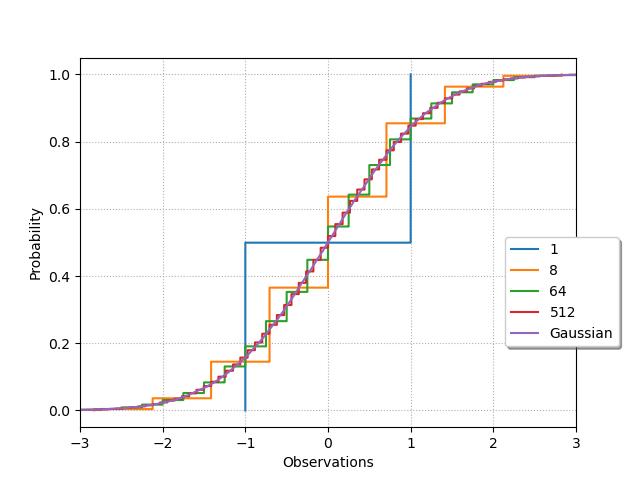
\includegraphics[max width=\textwidth]{image/Figure_2.png}
\end{center}


\end{document}